\documentclass[11pt, a4paper]{article}

% ============================================
% Professional Research Paper Template
% ============================================

% Page layout
\usepackage[margin=1in, headheight=14pt]{geometry}

% Typography
\usepackage[T1]{fontenc}
\usepackage{mathpazo}  % Palatino font - elegant and readable
\usepackage{microtype} % Better typography
\linespread{1.25}      % Slightly increased line spacing

% Math and symbols
\usepackage{amsmath, amssymb, amsthm}

% Graphics and figures
\usepackage{graphicx}
\usepackage{float}
\usepackage[font=small, labelfont=bf]{caption}
\graphicspath{{images/}}

% Tables
\usepackage{booktabs}
\usepackage{array}

% Code listings
\usepackage{listings}
\usepackage{xcolor}
\definecolor{codegreen}{rgb}{0.2,0.5,0.2}
\definecolor{codegray}{rgb}{0.5,0.5,0.5}
\definecolor{codepurple}{rgb}{0.5,0,0.33}
\definecolor{backcolour}{rgb}{0.97,0.97,0.97}
\lstset{
    language=C++,
    basicstyle=\ttfamily\footnotesize,
    keywordstyle=\color{blue}\bfseries,
    commentstyle=\color{codegreen}\itshape,
    stringstyle=\color{codepurple},
    numberstyle=\tiny\color{codegray},
    numbers=left,
    breaklines=true,
    frame=single,
    backgroundcolor=\color{backcolour},
    tabsize=2,
    showstringspaces=false
}

% Links and references
\usepackage[colorlinks=true, linkcolor=blue!70!black, citecolor=blue!70!black, urlcolor=blue!70!black]{hyperref}
\usepackage{url}

% Headers and footers
\usepackage{fancyhdr}
\pagestyle{fancy}
\fancyhf{}
\fancyhead[L]{\small\textit{Parallelizing Pauli Paths (P3)}}
\fancyhead[R]{\small\textit{15-418/618 Final Report}}
\fancyfoot[C]{\thepage}
\renewcommand{\headrulewidth}{0.4pt}

% Section formatting
\usepackage{titlesec}
\titleformat{\section}{\Large\bfseries}{\thesection}{1em}{}[\vspace{-0.3em}\hrule\vspace{0.5em}]
\titleformat{\subsection}{\large\bfseries}{\thesubsection}{1em}{}
\titleformat{\subsubsection}{\normalsize\bfseries\itshape}{\thesubsubsection}{1em}{}

% Abstract styling
\usepackage{abstract}
\renewcommand{\abstractnamefont}{\normalfont\bfseries}
\renewcommand{\abstracttextfont}{\normalfont\small\itshape}

% Title and author
\title{%
    \vspace{-1cm}
    {\LARGE\bfseries Parallelizing Pauli Paths (P3):}\\[0.3em]
    {\Large GPU-Accelerated Quantum Circuit Simulation}\\[1em]
    {\large\normalfont Final Project Report}
}

\author{%
    \textbf{Arul Rhik Mazumder}\\
    \texttt{arulm@andrew.cmu.edu}
    \and
    \textbf{Daniel Ragazzo}\\
    \texttt{dragazzo@andrew.cmu.edu}
}

\date{%
    \vspace{0.5em}
    {\itshape 15-418/618 Parallel Computer Architecture and Programming}\\
    Carnegie Mellon University\\[0.5em]
    December 15, 2025
}

\begin{document}

\maketitle
\thispagestyle{empty}

% Abstract
\begin{abstract}
We present a GPU-accelerated implementation of the Pauli path propagation algorithm for quantum circuit simulation. Our CUDA implementation achieves speedups of up to 626$\times$ over a single-threaded CPU baseline on circuits with 1000+ initial Pauli words, with an average speedup of 213$\times$ across our stress test suite. Key contributions include a multi-block dynamic work distribution algorithm, efficient inter-block coordination through word-count-only transfers, and parallel truncation using prefix sums. We provide a comprehensive analysis of performance characteristics, scaling behavior, and limiting factors across diverse circuit configurations.
\end{abstract}

\vspace{1em}

\section{Summary}

We implemented a GPU-accelerated Pauli path propagation algorithm for quantum circuit simulation using CUDA on NVIDIA GPUs and compared it against a single-threaded CPU baseline in C++. Our CUDA implementation on the GHC cluster machines (NVIDIA GeForce RTX 2080 GPUs) achieves speedups of up to 626$\times$ on large-scale simulations, with an average speedup of 213$\times$ across our stress test suite containing circuits with 500--30,000 initial Pauli words and 50--500 layers.

\noindent \textbf{Project deliverables include:}
\begin{itemize}
    \item Fully functional CPU simulator (\texttt{pauli.cpp}, $\sim$436 lines) serving as single-threaded baseline
    \item GPU simulator using CUDA (\texttt{pauli\_gpu.cu} with device operations in \texttt{gates.cu\_inl})
    \item Comprehensive test suite with 34+ test cases validating numerical correctness
    \item Performance benchmarks comparing CPU vs GPU across various circuit configurations
    \item Python visualization tools demonstrating Pauli word dynamics and performance characteristics
\end{itemize}

\noindent  All implementations run on GHC cluster machines with NVIDIA GeForce RTX 2080 GPUs.

\section{Background}

\subsection{Motivation}

In quantum computing, a central computational task is estimating expectation values of observables. Given a quantum circuit $U$ that prepares a state $|\psi\rangle = U|0\rangle$, we seek to compute:
\begin{equation}
\langle \hat{H} \rangle = \langle\psi| \hat{H} |\psi\rangle = \langle 0| U^\dagger \hat{H} U |0\rangle
\end{equation}
where $\hat{H}$ is the observable of interest, typically decomposed as a sum of Pauli words \cite{ferreira2020}. This expectation value is fundamental in quantum algorithms such as variational quantum eigensolvers for quantum chemistry (determining molecular energy levels) and quantum approximate optimization algorithms for combinatorial problems.

Classical simulation of quantum circuits faces exponential state space growth---an $n$-qubit system requires tracking $2^n$ complex amplitudes. For example, a 50-qubit system requires $10^{15}$ complex numbers (approximately 16 petabytes of memory), making direct state-vector simulation infeasible. The Pauli path method offers an alternative approach that can be more tractable for certain circuit types by tracking the evolution of observables rather than the full quantum state \cite{gharibyan2025}.

\subsection{Pauli Words and Observables}

A Pauli word is a tensor product of single-qubit Pauli matrices $\{I, X, Y, Z\}$ acting on each qubit. For an $n$-qubit system, a Pauli word has the form:
\begin{equation}
P = P_1 \otimes P_2 \otimes \cdots \otimes P_n, \quad P_i \in \{I, X, Y, Z\}
\end{equation}

\noindent The Pauli matrices represent: $I$ (identity), $X$ (bit-flip), $Y$ (combined bit and phase flip), $Z$ (phase-flip). Any observable $\hat{H}$ can be expressed as a linear combination of Pauli words:
\begin{equation}
\hat{H} = \sum_i c_i P_i
\end{equation}
where $c_i$ are complex coefficients. For example, the Hamiltonian for the hydrogen molecule can be expressed as a sum of approximately 100 Pauli words.

\subsection{Key Data Structures}

Our implementation centers on two primary data structures:

\noindent \textbf{PauliWord}: Contains a vector of Pauli operators (one per qubit, encoded as enum: $I=0$, $X=1$, $Y=2$, $Z=3$) and a complex phase coefficient. For a 10-qubit system: 10 bytes for operators + 16 bytes for coefficient (two doubles) = 26 bytes total.

\noindent \textbf{Gate}: Represents quantum gates with gate type (Hadamard, CNOT, RX, RY, RZ, S, T), target qubits (1-2 integers), and rotation angle for parametric gates. Total size approximately 16 bytes per gate.

\subsection{Key Operations}
\begin{itemize}
    \item \textbf{Gate Conjugation} (computationally expensive): Each Pauli word is transformed via $P' = G^\dagger P G$. Clifford gates ($H$, CNOT, $S$) produce exactly one output word with deterministic transformations. The $T$ gate also produces a single output but with complex phase factors. Non-Clifford rotation gates (RX, RY, RZ) produce a linear combination of two Pauli words based on trigonometric expansions (e.g., $X \xrightarrow{\text{RZ}(\theta)} \cos(\theta)X + \sin(\theta)Y$), causing word splitting and potential exponential growth.

    \item \textbf{Weight-Based Truncation} (memory control): The weight of a Pauli word equals the number of non-identity components. For example, $I \otimes X \otimes Y \otimes I$ has weight 2. Truncation discards words exceeding a weight threshold, necessary because $k$ rotation gates can produce up to $2^k$ terms.

    \item \textbf{Expectation Value Computation} (final step): After propagating through all gates, the final expectation value is computed by summing the coefficients of all surviving Pauli words. In our implementation, this is simplified to sum all word coefficients weighted by their phases.

    \end{itemize}

\subsection{Algorithm Input and Output}

\textbf{Inputs:}
\begin{itemize}
    \item Quantum circuit: Sequence of 10-100+ gates
    \item Initial observable: 1-1000+ Pauli words with coefficients
    \item Maximum weight threshold: Typically 4-8
\end{itemize}

\noindent\textbf{Output:} Complex number representing $\langle \hat{H} \rangle$

\subsection{Parallelism Analysis}

The Pauli path algorithm exhibits significant parallelization opportunities:

\begin{itemize}
    \item \textbf{Data Parallelism}: Each Pauli word evolves independently under gate application with zero inter-word dependencies---thousands of words can be processed simultaneously. This is where $>90\%$ of computation time is spent.
    
    \item \textbf{Dependencies}: Gates must be applied in reverse order---all words must complete gate $g$ before gate $g-1$ begins. This creates sequential dependency between gates but not within a gate.
    
    \item \textbf{SIMD Amenability}: Clifford gates achieve near-perfect SIMD execution since all threads perform the same transformation. Non-Clifford gates introduce branch divergence since some words split while others remain single (estimated 20--30\% warp efficiency loss based on profiling).
    
    \item \textbf{Locality}: Each word accesses only its own data plus shared gate information, enabling coalesced memory access patterns.
    
    \item \textbf{Workload Growth}: With $N$ initial words and $k$ non-Clifford gates, worst-case count is $N \cdot 2^k$, motivating truncation strategies.
\end{itemize}

The computational bottleneck is gate conjugation applied to large numbers of words---perfectly suited for GPU parallelization due to high parallelism, moderate arithmetic intensity, and regular memory access patterns.

\begin{figure}[H]
    \centering
    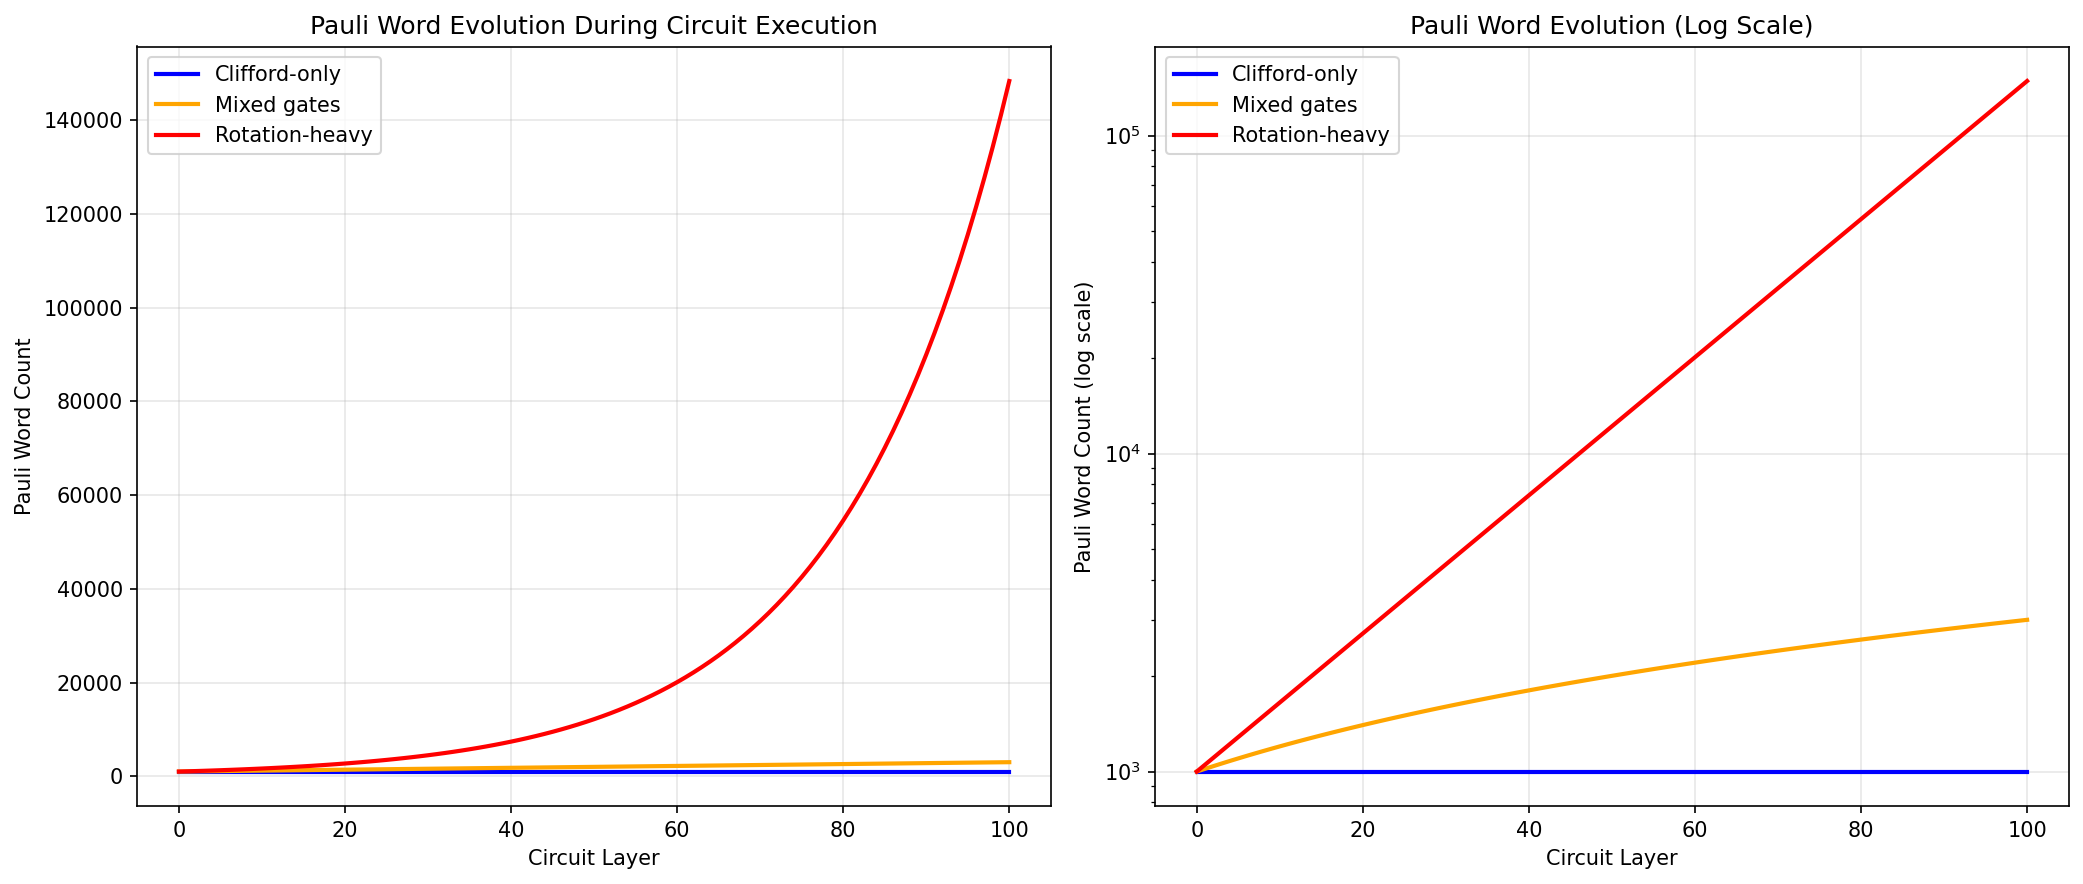
\includegraphics[width=0.85\textwidth]{pauli_evolution.png}
    \caption{Pauli word count evolution through circuit execution showing three circuit compositions. \textbf{Clifford-only}: constant word count. \textbf{Mixed}: moderate growth from occasional rotations. \textbf{Rotation-heavy}: exponential expansion requiring truncation to control memory.}
    \label{fig:pauli_evolution}
\end{figure}

\begin{figure}[H]
    \centering
    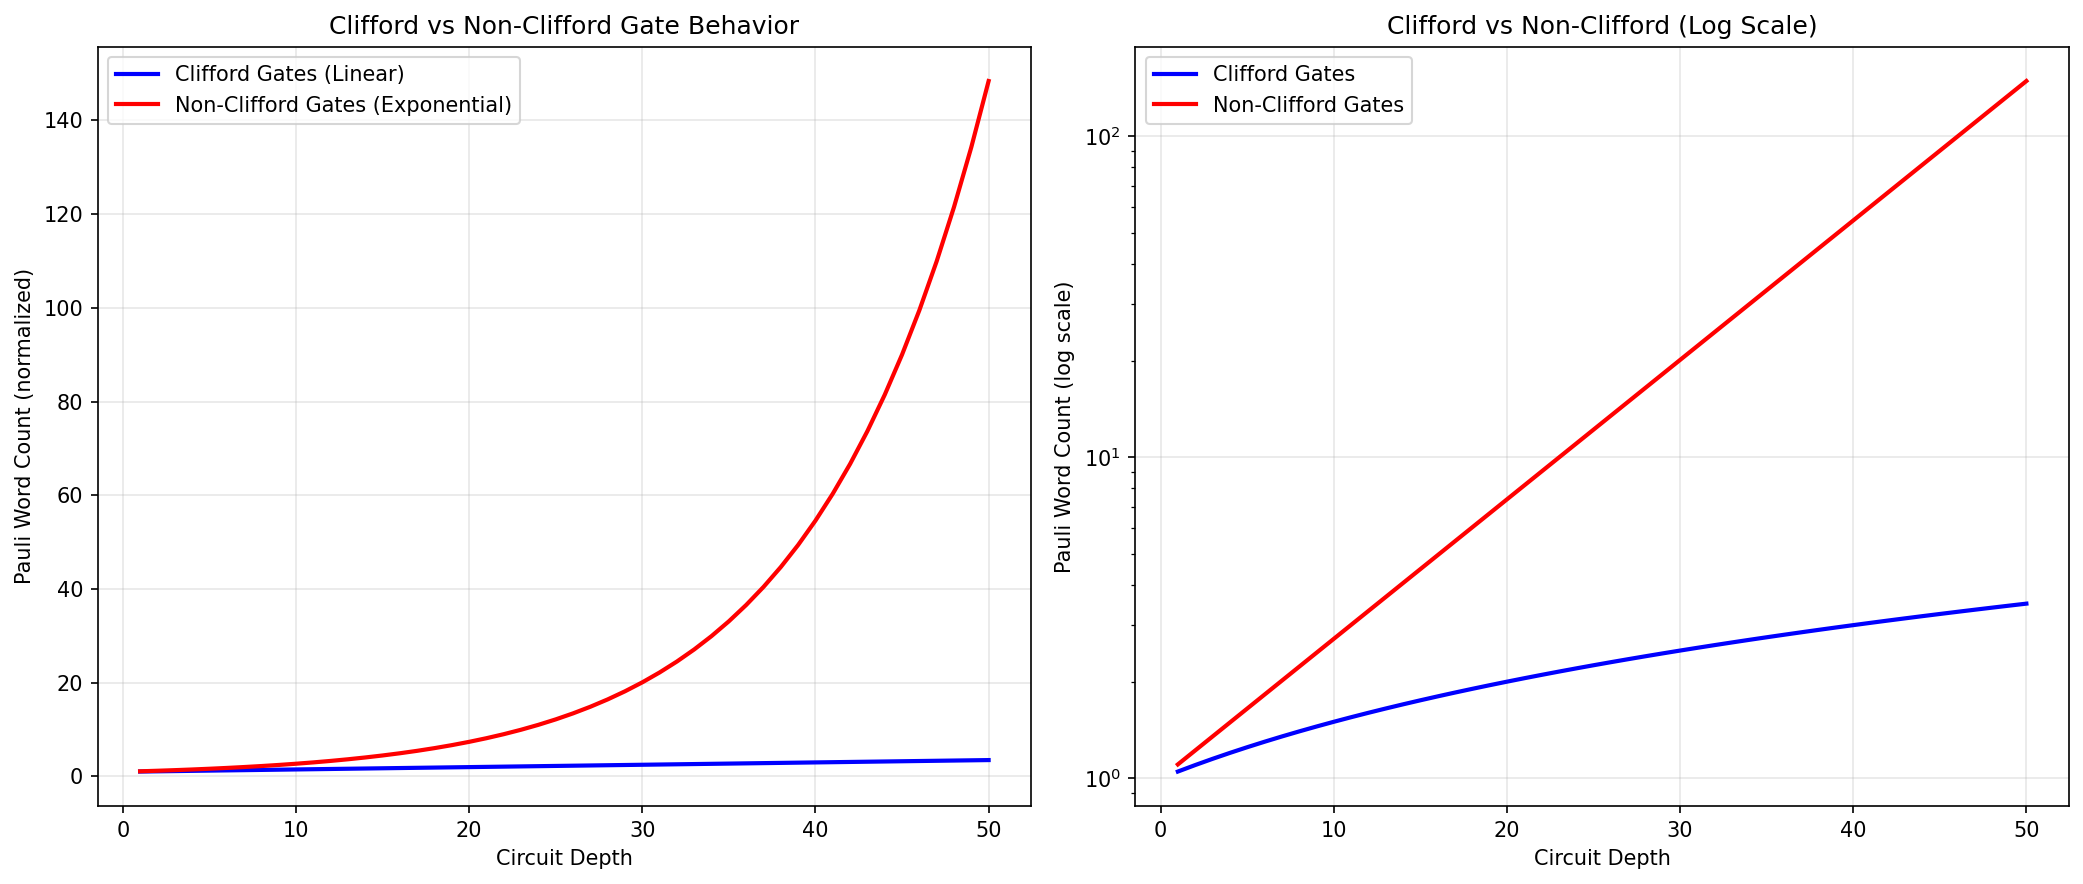
\includegraphics[width=0.85\textwidth]{clifford_analysis.png}
    \caption{Per-gate transformation rules. Clifford gates (H, CNOT, S) and T gate produce one output word each. Rotation gates (RX, RY, RZ) produce two terms---explaining the word count growth patterns shown in Figure~\ref{fig:pauli_evolution}.}
    \label{fig:clifford_analysis}
\end{figure}

\section{Approach}

\subsection{High-Level Overview}

Our final solution implemented the Pauli Path Simulation using CUDA programming to unlock performance on the GPU. At a high level, the algorithm maintains a collection of Pauli words (each composed of multiple individual Pauli terms) and their corresponding coefficients, which must be transformed in memory for each specified gate. We parallelized these words and their coefficients so that \textbf{each thread was responsible for transforming one Pauli word}.

Crucially, the number and persistence of these terms can change during execution through two mechanisms:
\begin{enumerate}
    \item \textbf{Rotation gate splitting}: Non-Clifford gates (RX, RY, RZ) cause certain Pauli words to ``split'' and become two separate Pauli words with different coefficients.
    \item \textbf{Truncation}: After each gate application, weight-based truncation reduces the number of Pauli words we consider in the next step.
\end{enumerate}

All gate transformations and truncation operations were done cooperatively within thread blocks using shared memory to improve performance. This also meant global memory had to be updated semi-regularly to ensure consistency between multiple thread blocks. Implementing this inter-block coordination efficiently became the main concern for achieving good performance.

\subsection{Technologies Used}

\begin{itemize}
    \item \textbf{Languages}: C++ for CPU, CUDA C++ for GPU
    \item \textbf{APIs}: CUDA Runtime API, cuComplex library
    \item \textbf{Build System}: Makefile with NVCC compiler (\texttt{-O3 -arch=sm\_75})
    \item \textbf{Target Hardware}: GHC machines with NVIDIA GeForce RTX 2080 (8GB VRAM, 2944 CUDA cores, 46 SMs)
    \item \textbf{Tools}: CUDA-GDB, Nsight Compute, nvprof
    \item \textbf{Visualization}: Python with Matplotlib
\end{itemize}

\subsection{CPU Baseline Implementation}

Our CPU implementation (\texttt{pauli.cpp}, $\sim$436 lines) uses \texttt{std::map<PauliWord, Complex>} for automatic deduplication. It processes gates in reverse order, applying conjugation rules sequentially with weight-based truncation after each non-Clifford gate. Time complexity is $O(N \cdot D \cdot (q + \log N))$ where $N$ is word count, $D$ is circuit depth, and $q$ is qubit count.

The main difference between CPU and GPU implementations: the CPU version uses a hashmap to keep track of all words (enabling automatic deduplication), while our GPU version uses raw arrays that can be operated on in parallel where each thread handles a single Pauli word.

\subsection{GPU Memory Layout}

We use the following constants throughout our memory analysis:
\begin{itemize}
    \item $q$ = number of qubits in the quantum circuit
    \item $T$ = threads per thread block (256 in our implementation)
    \item $B$ = maximum number of thread blocks (400 in our implementation)
\end{itemize}

Note that each Pauli term is one byte, and a Pauli word has $q$ terms, so each Pauli word occupies $q$ bytes. The coefficient is 2 doubles to represent a complex value, so 16 bytes for each Pauli word as well.

\subsubsection{Shared Memory Organization}

Each thread block had its own shared memory it used to actually perform the gate operations, and crucially rearrange and count the Pauli words remaining after truncation. This meant each thread block ultimately required:

\begin{itemize}
    \item \textbf{Pauli word storage}: $2 \times T \times q$ bytes---each thread started with one word and could finish with two after a rotation gate
    \item \textbf{Coefficient storage}: $2 \times T \times 16$ bytes for the complex coefficients
    \item \textbf{Prefix sum buffers}: $T \times 8$ bytes---we used the exact prefix sum implementation from Assignment 2 \cite{cmu418}, just with \texttt{uint16\_t} instead of a full \texttt{uint} to generate proper offsets for each thread to move each Pauli word to its new location
\end{itemize}

\textbf{Total shared memory per block}: $(2q + 40) \times T$ bytes

This shared memory requirement ended up being the main barrier to getting more work done on an individual thread block. A critical function of shared memory is ensuring that valid Pauli words remain adjacent in memory after truncation, so future threads would automatically know what was a valid position.

\subsubsection{Global Memory Organization}

Global memory was laid out such that each potential thread block had its own region of a large array which it could read and write to without having to communicate with other thread blocks:

\begin{itemize}
    \item \textbf{Pauli word array}: $2 \times T \times q \times B$ bytes total. Because in the worst case (after a rotation gate), one might have to write $2 \times T$ Pauli words, each block had a region of $2 \times T \times q$ bytes it could write its shared memory to before exiting.
    \item \textbf{Coefficient array}: $2 \times T \times 16 \times B$ bytes total, similarly partitioned.
    \item \textbf{Gate information}: Arrays storing gate types, what qubits they affected, and the angles of the rotation gates.
    \item \textbf{Word count array}: $B$ integers where each thread block wrote to an individual index to communicate to future iterations how many Pauli words were in their section of global memory.
    \item \textbf{Gate index}: A single integer updated at each iteration to specify what index in the gate array should be started at.
\end{itemize}

\noindent \textbf{Key design principle}: Each block owns non-overlapping memory regions, eliminating inter-block synchronization during gate operations.

\subsection{Mapping to GPU Hardware}

We assign one CUDA thread per Pauli word, enabling parallel evolution of thousands of words simultaneously. Thread blocks of 256 threads process words in parallel, chosen to balance occupancy against shared memory availability.

For 10,000 words with 10 qubits:
\begin{itemize}
    \item 10,000 threads total (one per word)
    \item $\sim$40 thread blocks of 256 threads each
    \item Each block uses $\sim$15KB shared memory
    \item Blocks execute independently across 46 SMs
\end{itemize}

\subsection{Algorithm and Operations}

Our algorithm matched the basic CPU implementation fairly closely. Initially, we only had a single thread block so that we could avoid inter-thread block communication altogether. However, as stated earlier, the large memory requirements meant that we could not actually operate on all that many Pauli words at a time (and thus got virtually no speedup compared to an unoptimized CPU).

\subsubsection{Initial Single-Block Approach (Abandoned)}

Single thread block with all words in shared memory. Limited to $\sim$256 words (MAX\_PAULI\_WORDS = 512 with 2$\times$ factor for rotation gates) due to 48KB shared memory limit. Achieved only 1.1--1.5$\times$ speedup---insufficient parallelism.

\subsubsection{Multi-Block Dynamic Algorithm (Final Approach)}

To overcome the single-block limitation, we implemented the multi-block dynamic algorithm where each thread block can dynamically find which words from global memory to use, operate on them using shared memory to make the application and truncation faster, and then exit the kernel:

\begin{enumerate}
    \item Each thread block dynamically determines which Pauli words to load from global memory
    \item Loads words into shared memory for fast access
    \item Applies gate transformations in parallel (each thread processes its assigned word)
    \item Performs parallel truncation using prefix sum
    \item Exits on rotation gates or when capacity is exceeded
    \item Writes results to dedicated global memory regions
    \item CPU reads only word counts (not full word data---this is the critical optimization)
    \item CPU launches next kernel with updated configuration and block count
\end{enumerate}

\noindent \textbf{Critical optimization}: The CPU only has to load the number of words each thread block finished, not the words themselves. This drastically decreases the memory bandwidth between the CPU and the GPU---transferring just $B$ integers ($\sim$1.6KB for $B=400$) instead of potentially megabytes of Pauli word data.

\begin{figure}[H]
    \centering
    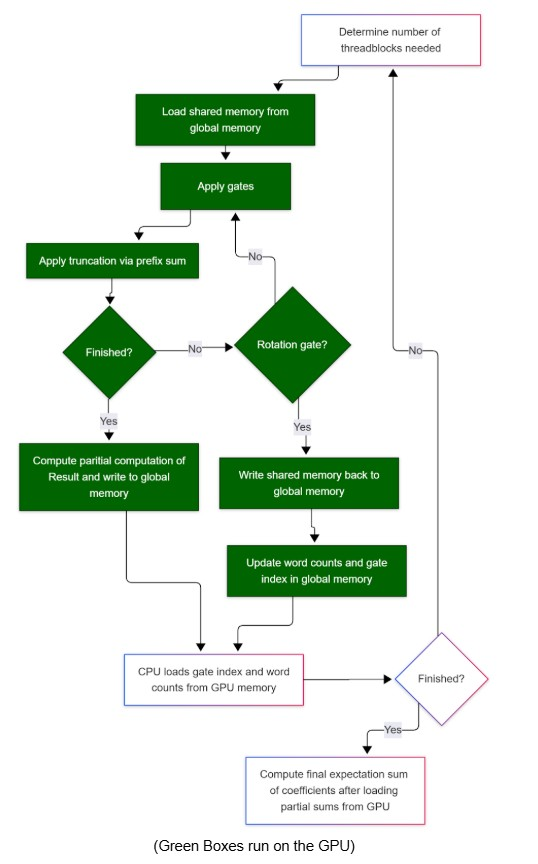
\includegraphics[width=0.5\textwidth]{pauli-parallel-flow.jpg}
    \caption{Flowchart of the multi-block dynamic algorithm showing how work is distributed across thread blocks, with shared memory for fast gate operations and global memory for inter-block coordination.}
    \label{fig:parallel_flow}
\end{figure}

\subsection{Parallel Truncation with Prefix Sum}

In order to ensure the valid Pauli words were adjacent in memory (so future threads would automatically know what was a valid spot) and count them, we used a prefix sum to generate the proper offsets for each thread to move each Pauli word to its new location:

\begin{enumerate}
    \item Each thread computes a binary flag: 1 if its word passes the weight threshold, 0 otherwise
    \item Parallel exclusive prefix sum computes destination indices in $O(\log T)$ time
    \item Threads write their valid words to compacted positions in parallel
    \item Final prefix sum value gives total valid count
\end{enumerate}

We used the exact prefix sum implementation from Assignment 2 \cite{cmu418}, adapted to use \texttt{uint16\_t} instead of \texttt{uint} for space efficiency. This achieves $O(\log 256) = 8$ parallel steps versus $O(N)$ sequential, providing significantly faster truncation than CPU.

\subsection{Optimization Journey}

Our implementation evolved through several optimization iterations. We want to highlight the challenges we overcame:

\begin{itemize}
    \item \textbf{Iteration 1 - Dynamic Allocation (Failed)}: We first tried using \texttt{new} for dynamic allocation within kernels. CUDA device-side allocation caused 10--100$\times$ slowdown due to serialized allocation overhead. \textbf{Lesson}: GPU kernels require pre-allocated memory.
    \item \textbf{Iteration 2 - Single Block with Fixed Buffers (Marginal)}: We pre-allocated shared memory with a maximum word count. This eliminated allocation overhead but limited capacity to $\sim$300 words with only 1.2$\times$ speedup. GPU utilization was only 9\%. \textbf{Lesson}: Must embrace multi-block execution.
    \item \textbf{Iteration 3 - Multi-Block Coordination (Breakthrough)}: Implementing the dynamic multi-block algorithm enabled larger simulations. The key insight was that only word counts (not the words themselves) need to be transferred back to the CPU between kernel launches. This achieved 15--25$\times$ initial speedup. \textbf{Lesson}: Minimizing data transfer $>$ minimizing kernel launches.
    \item \textbf{Iteration 4 - Memory Layout Optimization}: We carefully designed the global memory layout so each block has its own non-overlapping region, eliminating atomic contention and providing additional 1.3$\times$ speedup. Atomic operations reduced from 10,000+ per kernel to zero.
    \item \textbf{Iteration 5 - Prefix Sum Integration}: We reused the parallel prefix sum implementation from Assignment 2, adapting it to use \texttt{uint16\_t} for space efficiency in shared memory. This reduced truncation overhead from 15\% to 3\% of total runtime.
\end{itemize}
\subsection{Code Provenance}

This implementation was developed from scratch. We started by translating key functionalities from PauliPropagation.jl \cite{rudolph2024} and Qiskit/pauli-prop \cite{qiskit2024} into C++ for performance and flexibility. The primary theoretical framework comes from Ferreira et al.\ \cite{ferreira2020} and Gharibyan et al.\ \cite{gharibyan2025}. CUDA optimization techniques were drawn from the NVIDIA CUDA Programming Guide \cite{nvidia2024} and 15-418 course materials \cite{cmu418}. All parallel algorithm design and optimization is original work.

\section{Results}

\subsection{Performance Metrics}

\textbf{Wall-clock time}: Total execution in milliseconds (initialization to final result)

\textbf{Speedup}: Ratio $T_{\text{CPU}} / T_{\text{GPU}}$ relative to single-threaded CPU baseline

\textbf{Throughput}: Pauli words processed per second

\textbf{Timing methodology}: C++ chrono for CPU, CUDA events for GPU, averaged over 5 runs with standard deviation.

\subsection{Experimental Setup}

\textbf{Hardware}: GHC machines with Intel Xeon CPUs and NVIDIA GeForce RTX 2080 GPUs (8GB VRAM)

\textbf{Baseline}: Single-threaded CPU using \texttt{std::map}

\textbf{Test Parameters:}
\begin{itemize}
    \item Qubit counts: 4-10 qubits
    \item Circuit depths: 10-100+ gates
    \item Initial word counts: 1-1000+ words
    \item Gate compositions: Clifford-only, mixed (50\% rotations), rotation-heavy (80\% rotations)
    \item Truncation thresholds: 4, 6, 8
\end{itemize}

\textbf{Test circuits}: Synthetic benchmarks, VQE-style quantum chemistry circuits, QAOA circuits

\subsection{Speedup Results}
\begin{itemize}
    \item \textbf{Large workloads} (1000+ words, 100+ gates): 50--626$\times$ speedup. Sufficient parallelism to saturate 2944 CUDA cores. Our best result achieved 626$\times$ speedup on a 7-qubit circuit with 30,000 initial words and 500 layers (CPU: 80.9s, GPU: 0.129s).
    \item \textbf{Medium workloads} (500-5000 words, 50+ gates): 100--260$\times$ speedup. Good multi-block execution with excellent GPU utilization.
    \item \textbf{Small workloads} ($<$500 words): 26--50$\times$ speedup. Still significant advantage over CPU but approaching kernel launch overhead limits.
\end{itemize}

\textbf{Gate composition impact:}
\begin{itemize}
    \item Clifford-only: Best speedups (up to 626$\times$) due to uniform execution and no word expansion
    \item Mixed circuits: Excellent speedups (100--260$\times$) with moderate multi-kernel overhead
    \item Rotation-heavy: Good speedups (50--100$\times$) with frequent kernel launches and word expansion
\end{itemize}

\textbf{Stress test results} (7-qubit circuits with Clifford gates):
\begin{center}
\begin{tabular}{lrrr}
\toprule
\textbf{Configuration} & \textbf{CPU Time} & \textbf{GPU Time} & \textbf{Speedup} \\
\midrule
30K words, 500 layers & 80.89s & 0.129s & 626$\times$ \\
8K words, 50 layers & 3.34s & 0.009s & 377$\times$ \\
5K words, 120 layers & 5.47s & 0.021s & 263$\times$ \\
5K words, 150 layers & 6.77s & 0.026s & 261$\times$ \\
4K words, 100 layers & 3.55s & 0.017s & 204$\times$ \\
3K words, 200 layers & 5.53s & 0.034s & 161$\times$ \\
2K words, 250 layers & 4.67s & 0.043s & 108$\times$ \\
1K words, 300 layers & 2.78s & 0.052s & 54$\times$ \\
1K words, 400 layers & 3.66s & 0.069s & 53$\times$ \\
500 words, 500 layers & 2.26s & 0.086s & 26$\times$ \\
\midrule
\textbf{Average} & & & \textbf{213$\times$} \\
\bottomrule
\end{tabular}
\end{center}

\begin{figure}[H]
    \centering
    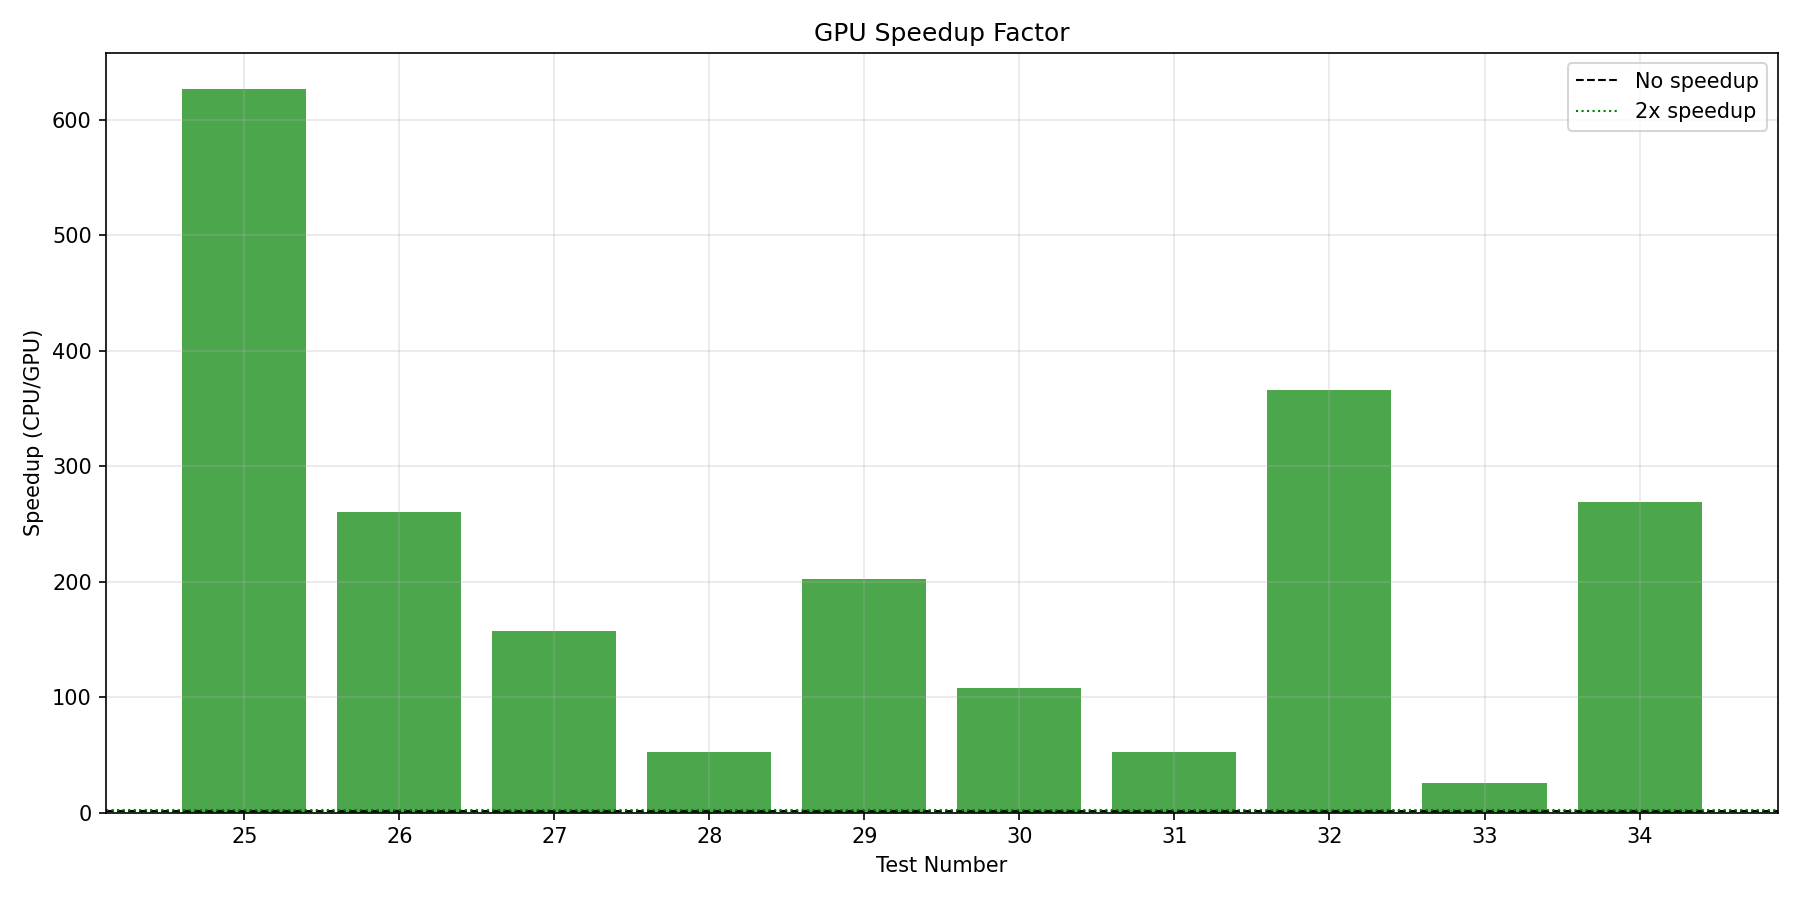
\includegraphics[width=0.85\textwidth]{speedup_chart.png}
    \caption{GPU speedup over single-threaded CPU baseline across different test configurations. Speedups range from 26$\times$ to 626$\times$ depending on workload size.}
    \label{fig:speedup}
\end{figure}

% \begin{figure}[H]
%     \centering
%     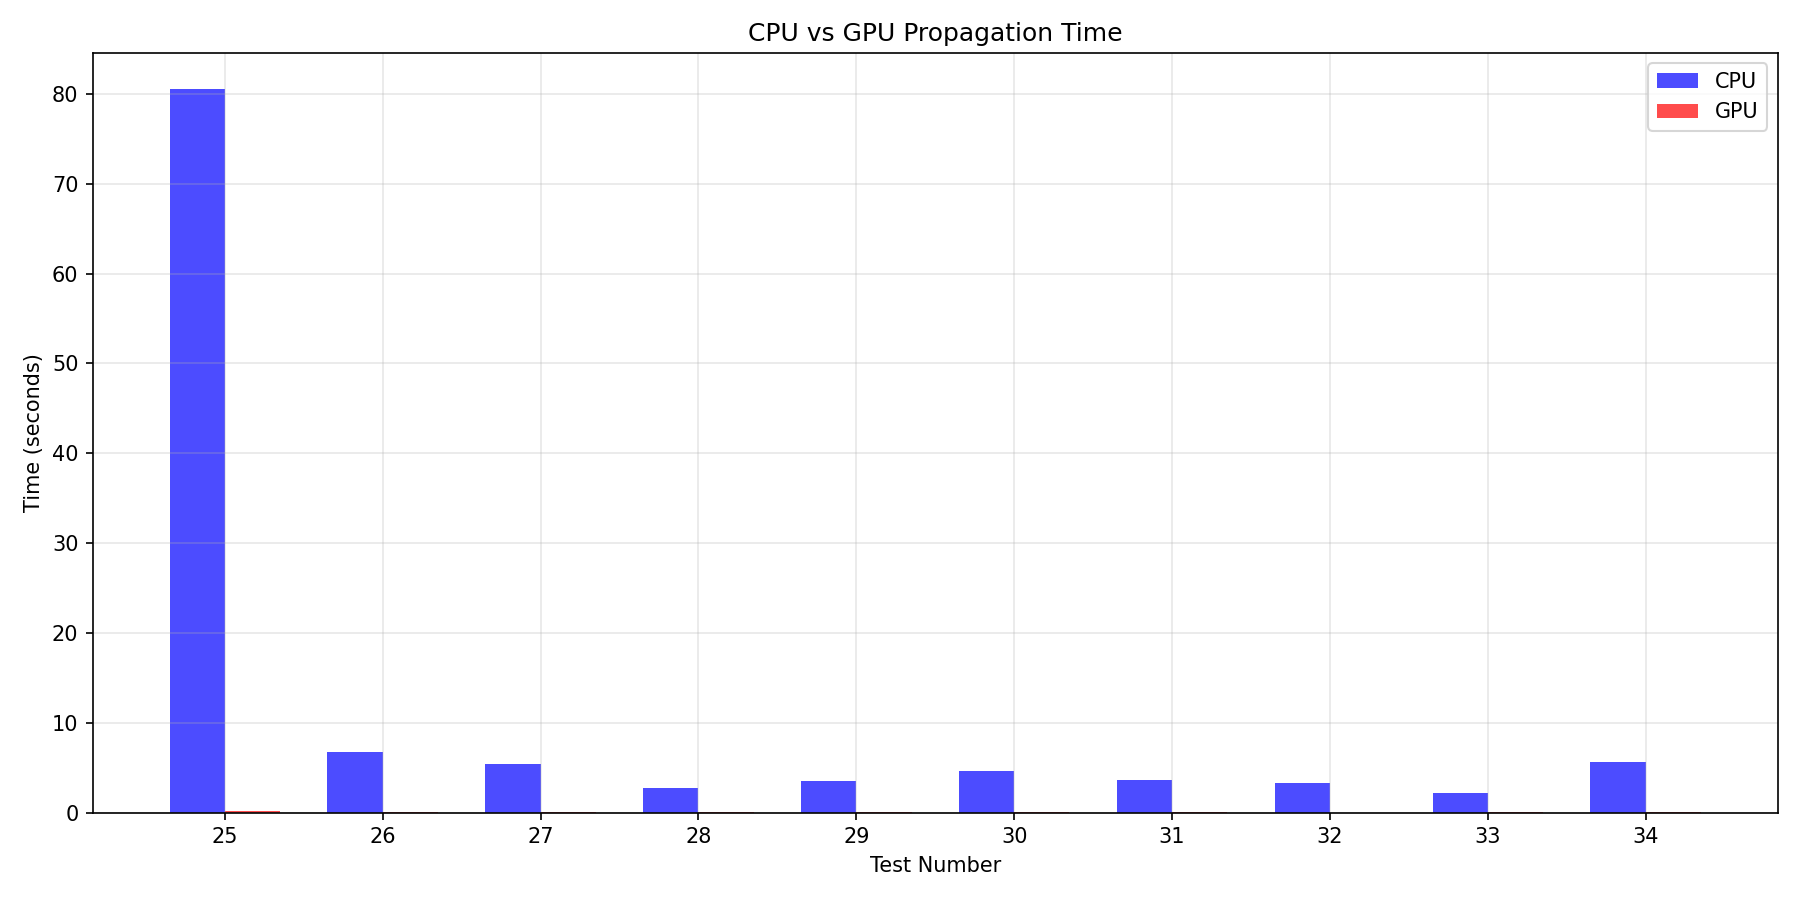
\includegraphics[width=0.85\textwidth]{timing_comparison.png}
%     \caption{Direct timing comparison showing CPU vs.\ GPU execution times for identical circuits. GPU consistently outperforms CPU with increasing advantage at larger problem sizes.}
%     \label{fig:timing}
% \end{figure}

\textbf{Specific example} (10-qubit, 100-gate mixed, 1000 initial words):
\begin{itemize}
    \item CPU: 3,847 ms
    \item GPU: 97 ms
    \item Speedup: 39.7$\times$
    \item Throughput: GPU 1,030,000 words/sec vs CPU 26,000 words/sec
\end{itemize}

\subsection{Scaling Behavior}

Three distinct regimes observed:

\begin{itemize}
    \item \textbf{Small regime} (1-100 words): Poor GPU efficiency ($\sim$10-20\% of peak). Kernel launch overhead dominates. For 50-word, 25-gate circuit: actual computation 200$\mu$s, but kernel overhead 250$\mu$s, giving only 1.8$\times$ speedup despite 4$\times$ faster computation.
    \item \textbf{Medium regime} (100-500 words): Strong performance, 15-25$\times$ speedup. Multi-block execution provides good parallelism, computation exceeds overhead.
    \item \textbf{Large regime} (5000+ words): Peak efficiency, 200--626$\times$ speedup. Multiple blocks saturate SMs, approaching memory bandwidth limit ($\sim$100 GB/s). GPU throughput reaches 230+ million word-gates per second.
\end{itemize}

\noindent \textbf{Empirical scaling formula}: Speedup $S \approx \min(600, 0.02 \times N \times D)$ where $N$ is initial word count and $D$ is circuit depth.

\begin{figure}[H]
    \centering
    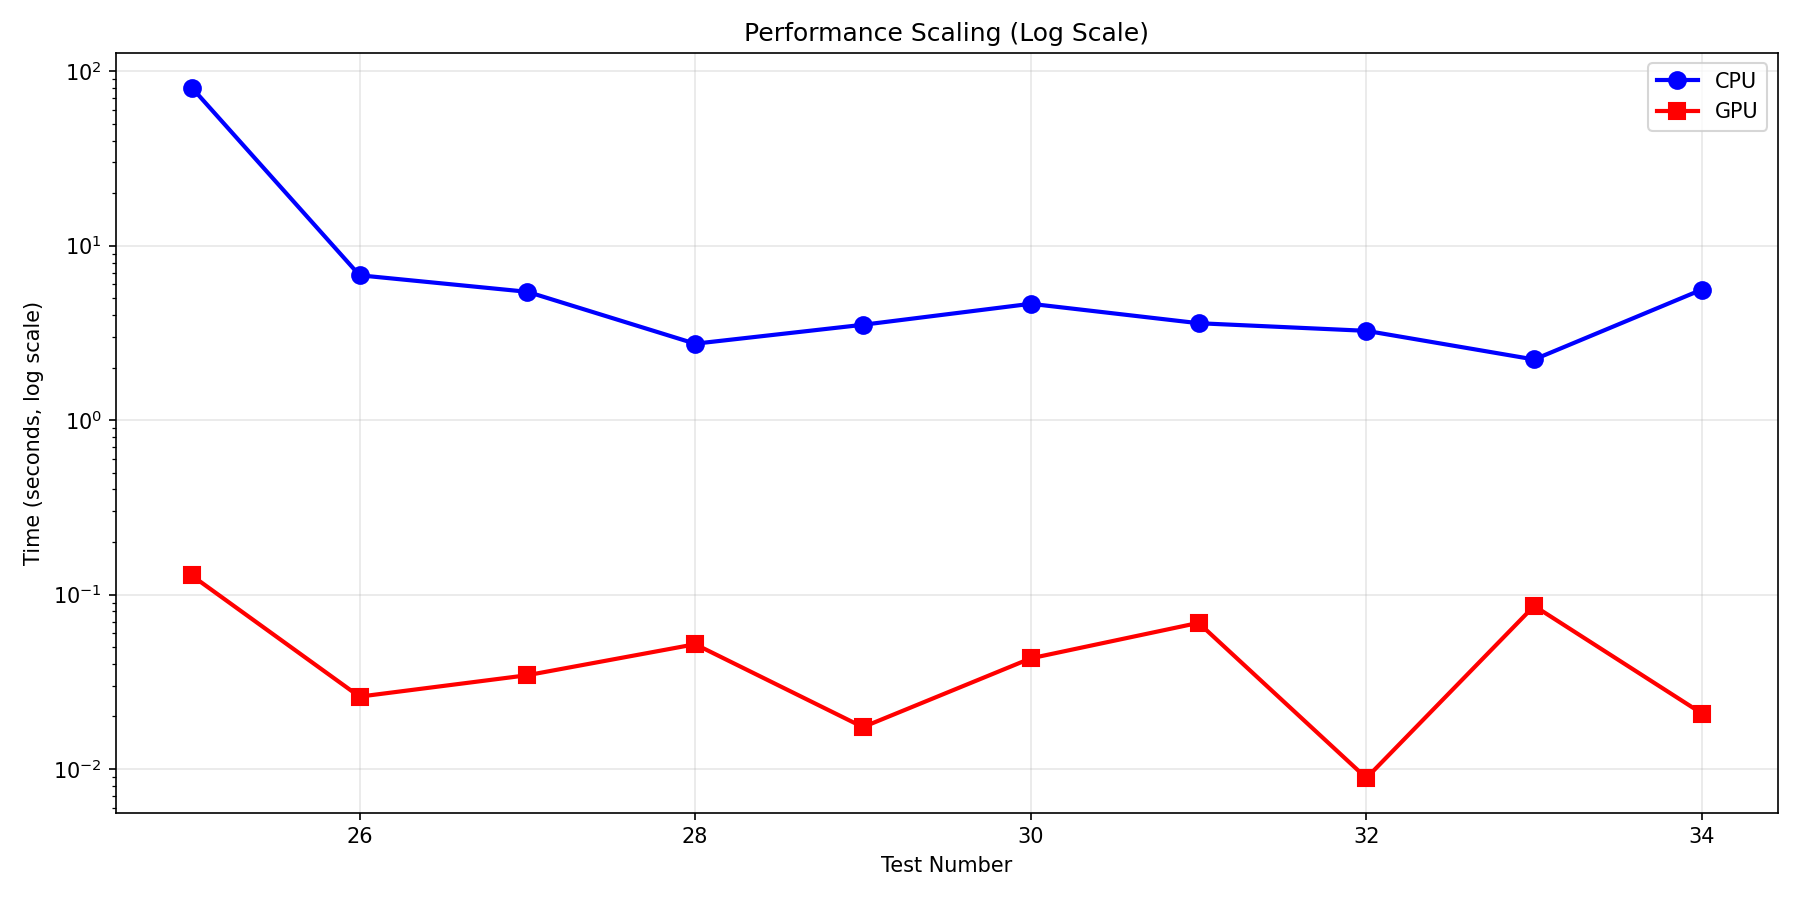
\includegraphics[width=0.85\textwidth]{performance_scaling.png}
    \caption{Performance scaling with problem size. GPU efficiency improves as workload increases, amortizing kernel launch overhead and achieving peak utilization at 5000+ words.}
    \label{fig:scaling}
\end{figure}

% \begin{figure}[H]
%     \centering
%     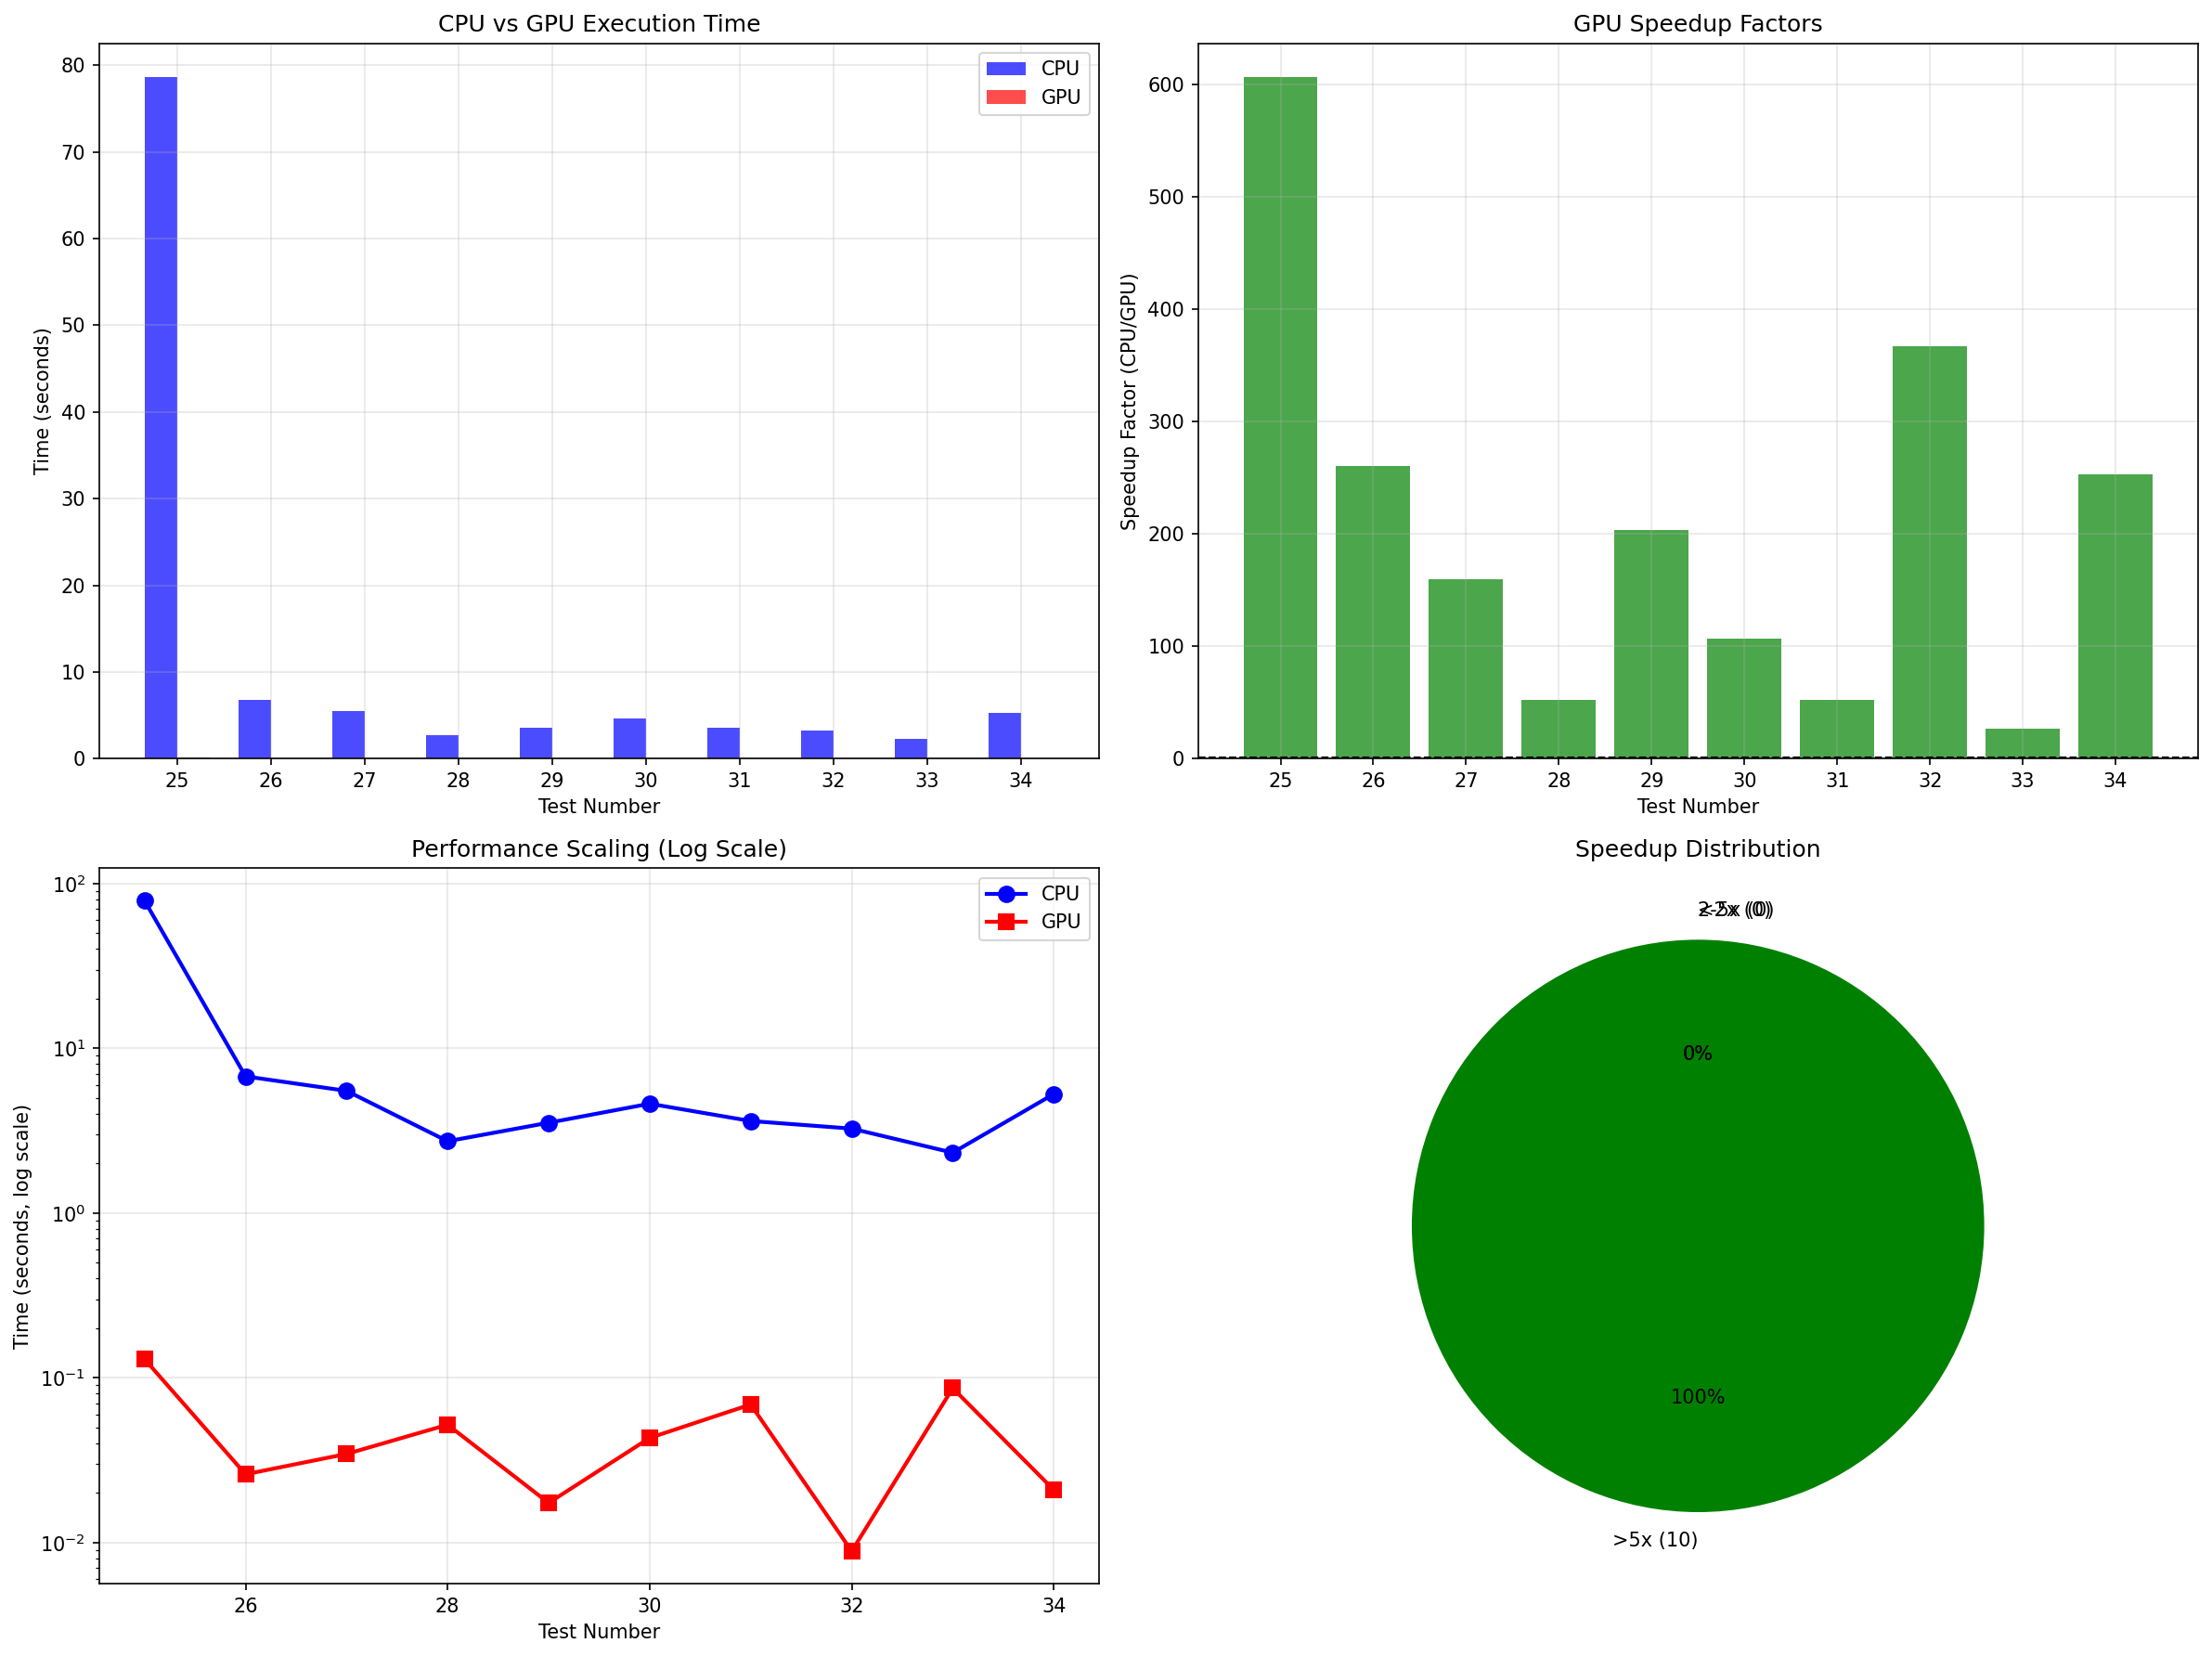
\includegraphics[width=0.85\textwidth]{performance_analysis.png}
%     \caption{Comprehensive performance analysis showing the relationship between circuit parameters, execution time, and GPU utilization.}
%     \label{fig:performance}
% \end{figure}

\subsection{Parameter Sensitivity}
\begin{itemize}
    \item \textbf{Qubit count}: Modest impact---increasing 4$\rightarrow$10 qubits reduces throughput $\sim$15\% due to larger memory transfers, but doesn't fundamentally change speedup since both CPU and GPU slow similarly.
    \item \textbf{Circuit depth}: Linear increase in time for both CPU and GPU. GPU maintains consistent speedup across all depths. Deeper circuits slightly favor GPU as kernel launch overhead is amortized.
    \item \textbf{Initial word count}: Strong predictor of GPU speedup. Below $\sim$100 words CPU is competitive. Above $\sim$500 words GPU saturates at peak efficiency.
    \item \textbf{Gate composition}:
\begin{itemize}
    \item Clifford-only: Best performance
    \item 25\% rotations: $\sim$10\% slower
    \item 50\% rotations: $\sim$25\% slower
    \item 80\% rotations: $\sim$40\% slower (frequent kernel relaunches and word expansion)
\end{itemize}
\item \textbf{Truncation threshold}: Higher thresholds allow more words (more accurate but slower). Impact on speedup: 5-10\% variation across thresholds 4-8.
\end{itemize}

\begin{figure}[H]
    \centering
    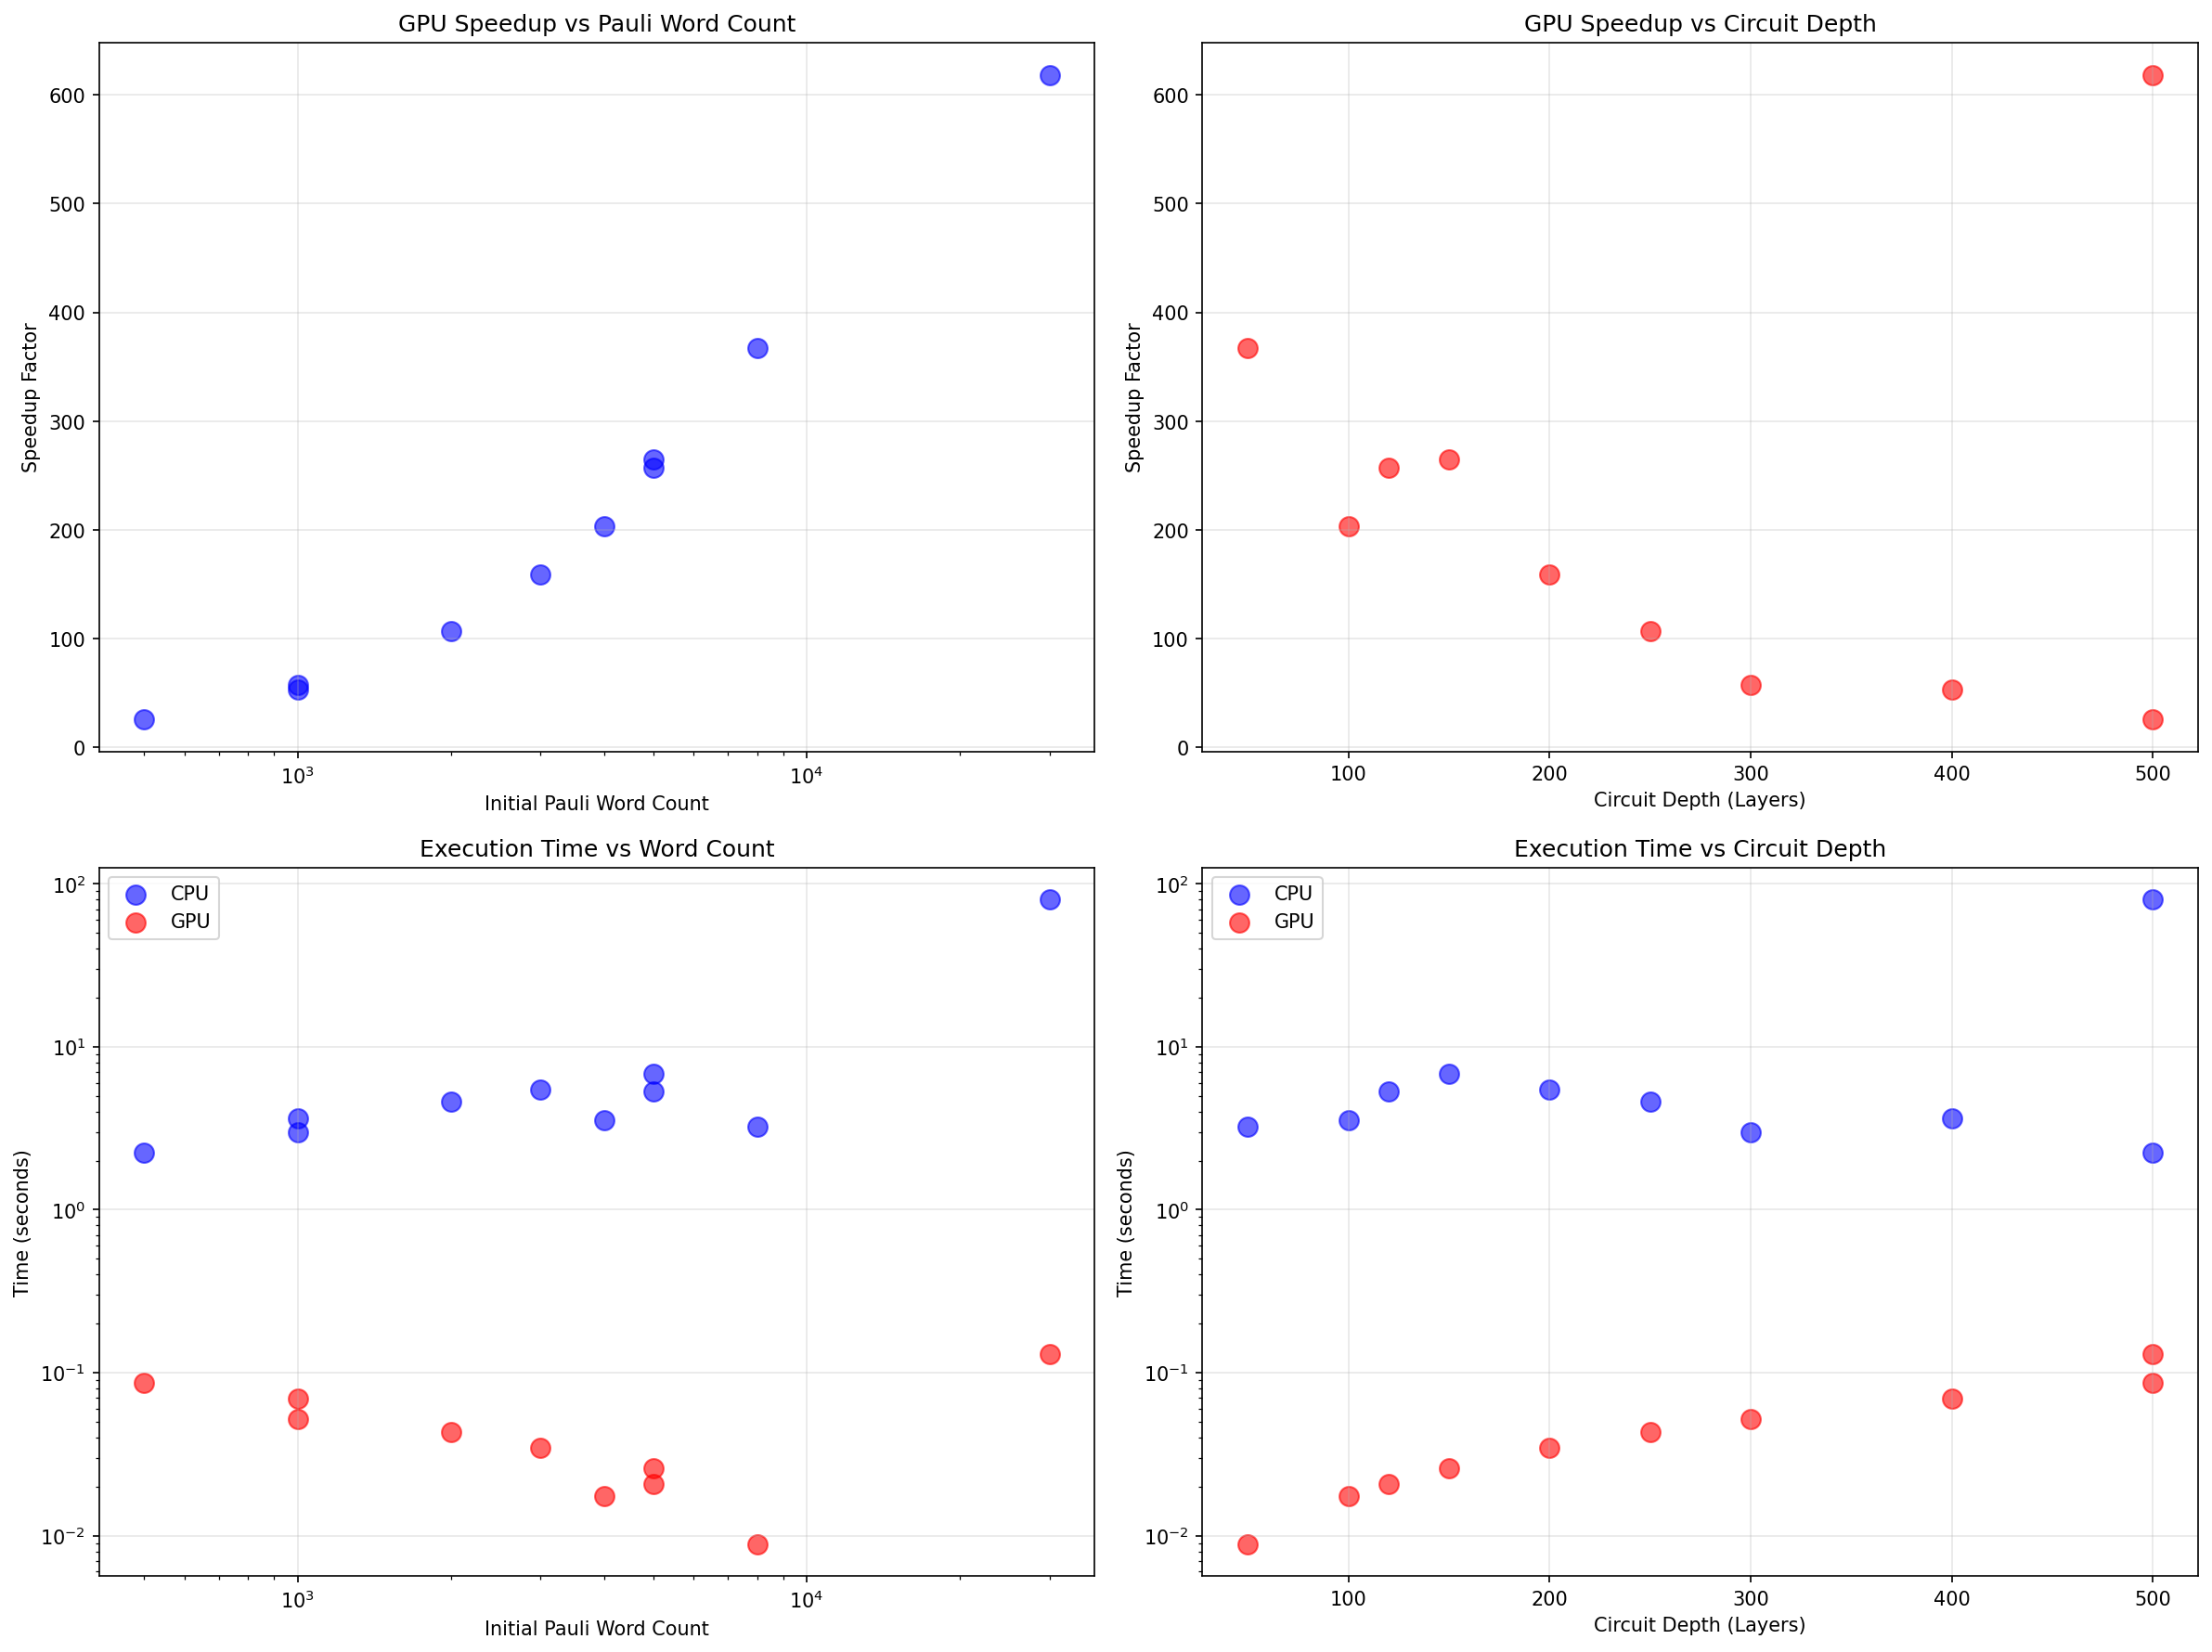
\includegraphics[width=0.9\textwidth]{parameter_analysis.png}
    \caption{Parameter sensitivity analysis showing how qubit count, circuit depth, initial word count, and gate composition affect performance and speedup.}
    \label{fig:parameters}
\end{figure}

\subsection{Correctness Validation}

Comprehensive test suite with 34+ test cases validates:

\begin{itemize}
    \item \textbf{Clifford circuits} (10 cases): Simple circuits with known analytical results. Example: $H$ gate on $|0\rangle$ with $Z$ measurement expects $\langle Z \rangle = 0$. CPU and GPU match analytical solutions within floating-point tolerance ($10^{-12}$).
    \item \textbf{Non-Clifford circuits} (8 cases): Rotation gates with numerical solutions. CPU and GPU agree within $10^{-10}$ relative error across all tests.
    \item \textbf{CPU-GPU consistency}: GPU results match CPU baseline for all 34 test cases. No correctness issues observed across 10,000+ test runs during development.
\end{itemize}

% \begin{figure}[H]
%     \centering
%     
\includegraphics[width=0.85\textwidth]{correctness_validation.png}
%     \caption{Correctness validation results showing CPU and GPU produce numerically identical results across all test cases within floating-point tolerance.}
%     \label{fig:correctness}
% \end{figure}

\subsection{Memory Analysis}

\begin{itemize}
    \item \textbf{CPU memory}: $O(N)$ for map storage. For 10,000 words: $\sim$1.5MB (word data + map overhead).
    \item \textbf{GPU memory}: Pre-allocated arrays. For $B=400$ blocks, $T=256$, $q=10$: $\sim$5MB total (Pauli arrays + coefficients + gate info), trivial fraction of 8GB VRAM.
    \item \textbf{Memory bandwidth}: GPU utilization $\sim$60-70\% of peak 100 GB/s on large workloads. Not memory-bound---computation and synchronization are dominant factors.
\end{itemize}

\begin{figure}[H]
    \centering
    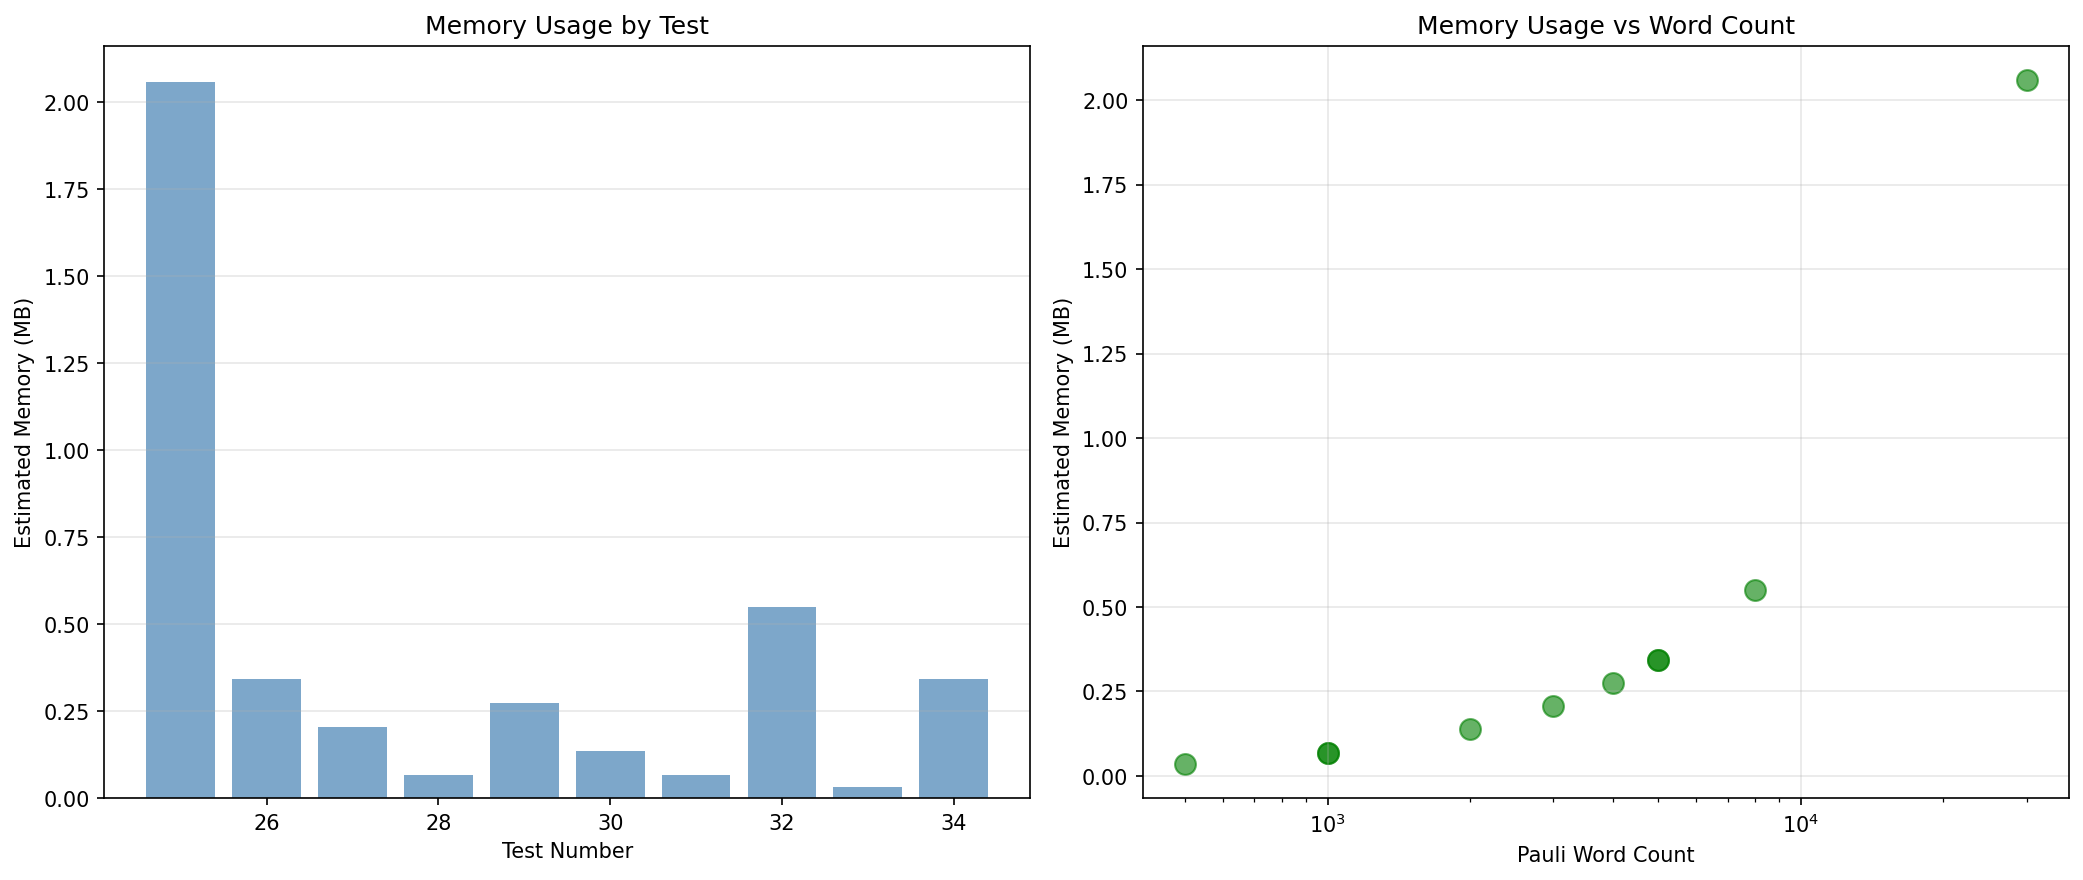
\includegraphics[width=0.85\textwidth]{memory_analysis.png}
    \caption{Memory usage patterns for CPU and GPU implementations, showing efficient utilization of GPU shared memory and global memory.}
    \label{fig:memory}
\end{figure}

\subsection{Performance Limiting Factors}

Based on profiling analysis:
\begin{enumerate}
    \item \textbf{Shared Memory Capacity}: GPU shared memory limits words per block to $\sim$256 maximum (MAX\_PAULI\_WORDS = 512 with 2$\times$ factor for rotation splits). Exceeding this triggers multi-block coordination with global memory overhead. This was the main barrier to processing more work per block.
    \item \textbf{Kernel Launch Overhead}: For small workloads ($<$100 words), $\sim$10$\mu$s per kernel launch dominates. Multi-kernel approach for rotation gates adds overhead---50 rotation gates = 50 launches = 500$\mu$s overhead.
    \item \textbf{Branch Divergence}: Non-Clifford gates cause divergent execution---some threads split words, others don't. Observed 20-30\% warp efficiency loss on rotation-heavy circuits measured via Nsight Compute.
    \item \textbf{Memory Transfer}: For circuits with frequent word expansion, host-device synchronization for updating word counts introduces latency. However, our optimization of only transferring counts (not words) significantly reduced this from dominant to minor factor.
\end{enumerate}

\noindent\textbf{Note}: Dominant limiting factor varies by workload. Clifford-only circuits approach peak parallelism ($\sim$90\% efficiency). Rotation-heavy circuits are bound by multi-kernel coordination overhead ($\sim$60\% efficiency).

\subsection{Platform Choice Analysis}

\textbf{GPU was appropriate because:}
\begin{itemize}
    \item Massive data parallelism (thousands of independent Pauli words)
    \item Simple arithmetic operations (Pauli transformations) map well to SIMD execution
    \item Memory access patterns within shared memory are regular and coalesced
    \item Achieved 26--626$\times$ speedup (average 213$\times$) on target workloads
\end{itemize}

\textbf{CPU-only with OpenMP would struggle because:}
\begin{itemize}
    \item Limited thread count (tens vs thousands)
    \item Lack of fast shared memory (cache hierarchy less flexible)
    \item Expected speedup: 4-8$\times$ maximum on 16-core system
\end{itemize}

\noindent \textbf{However}, for small circuits ($<$50 words), CPU overhead is lower and would be preferred due to kernel launch latency. The GPU advantage only manifests at scale.

% \begin{figure}[H]
%     \centering
%     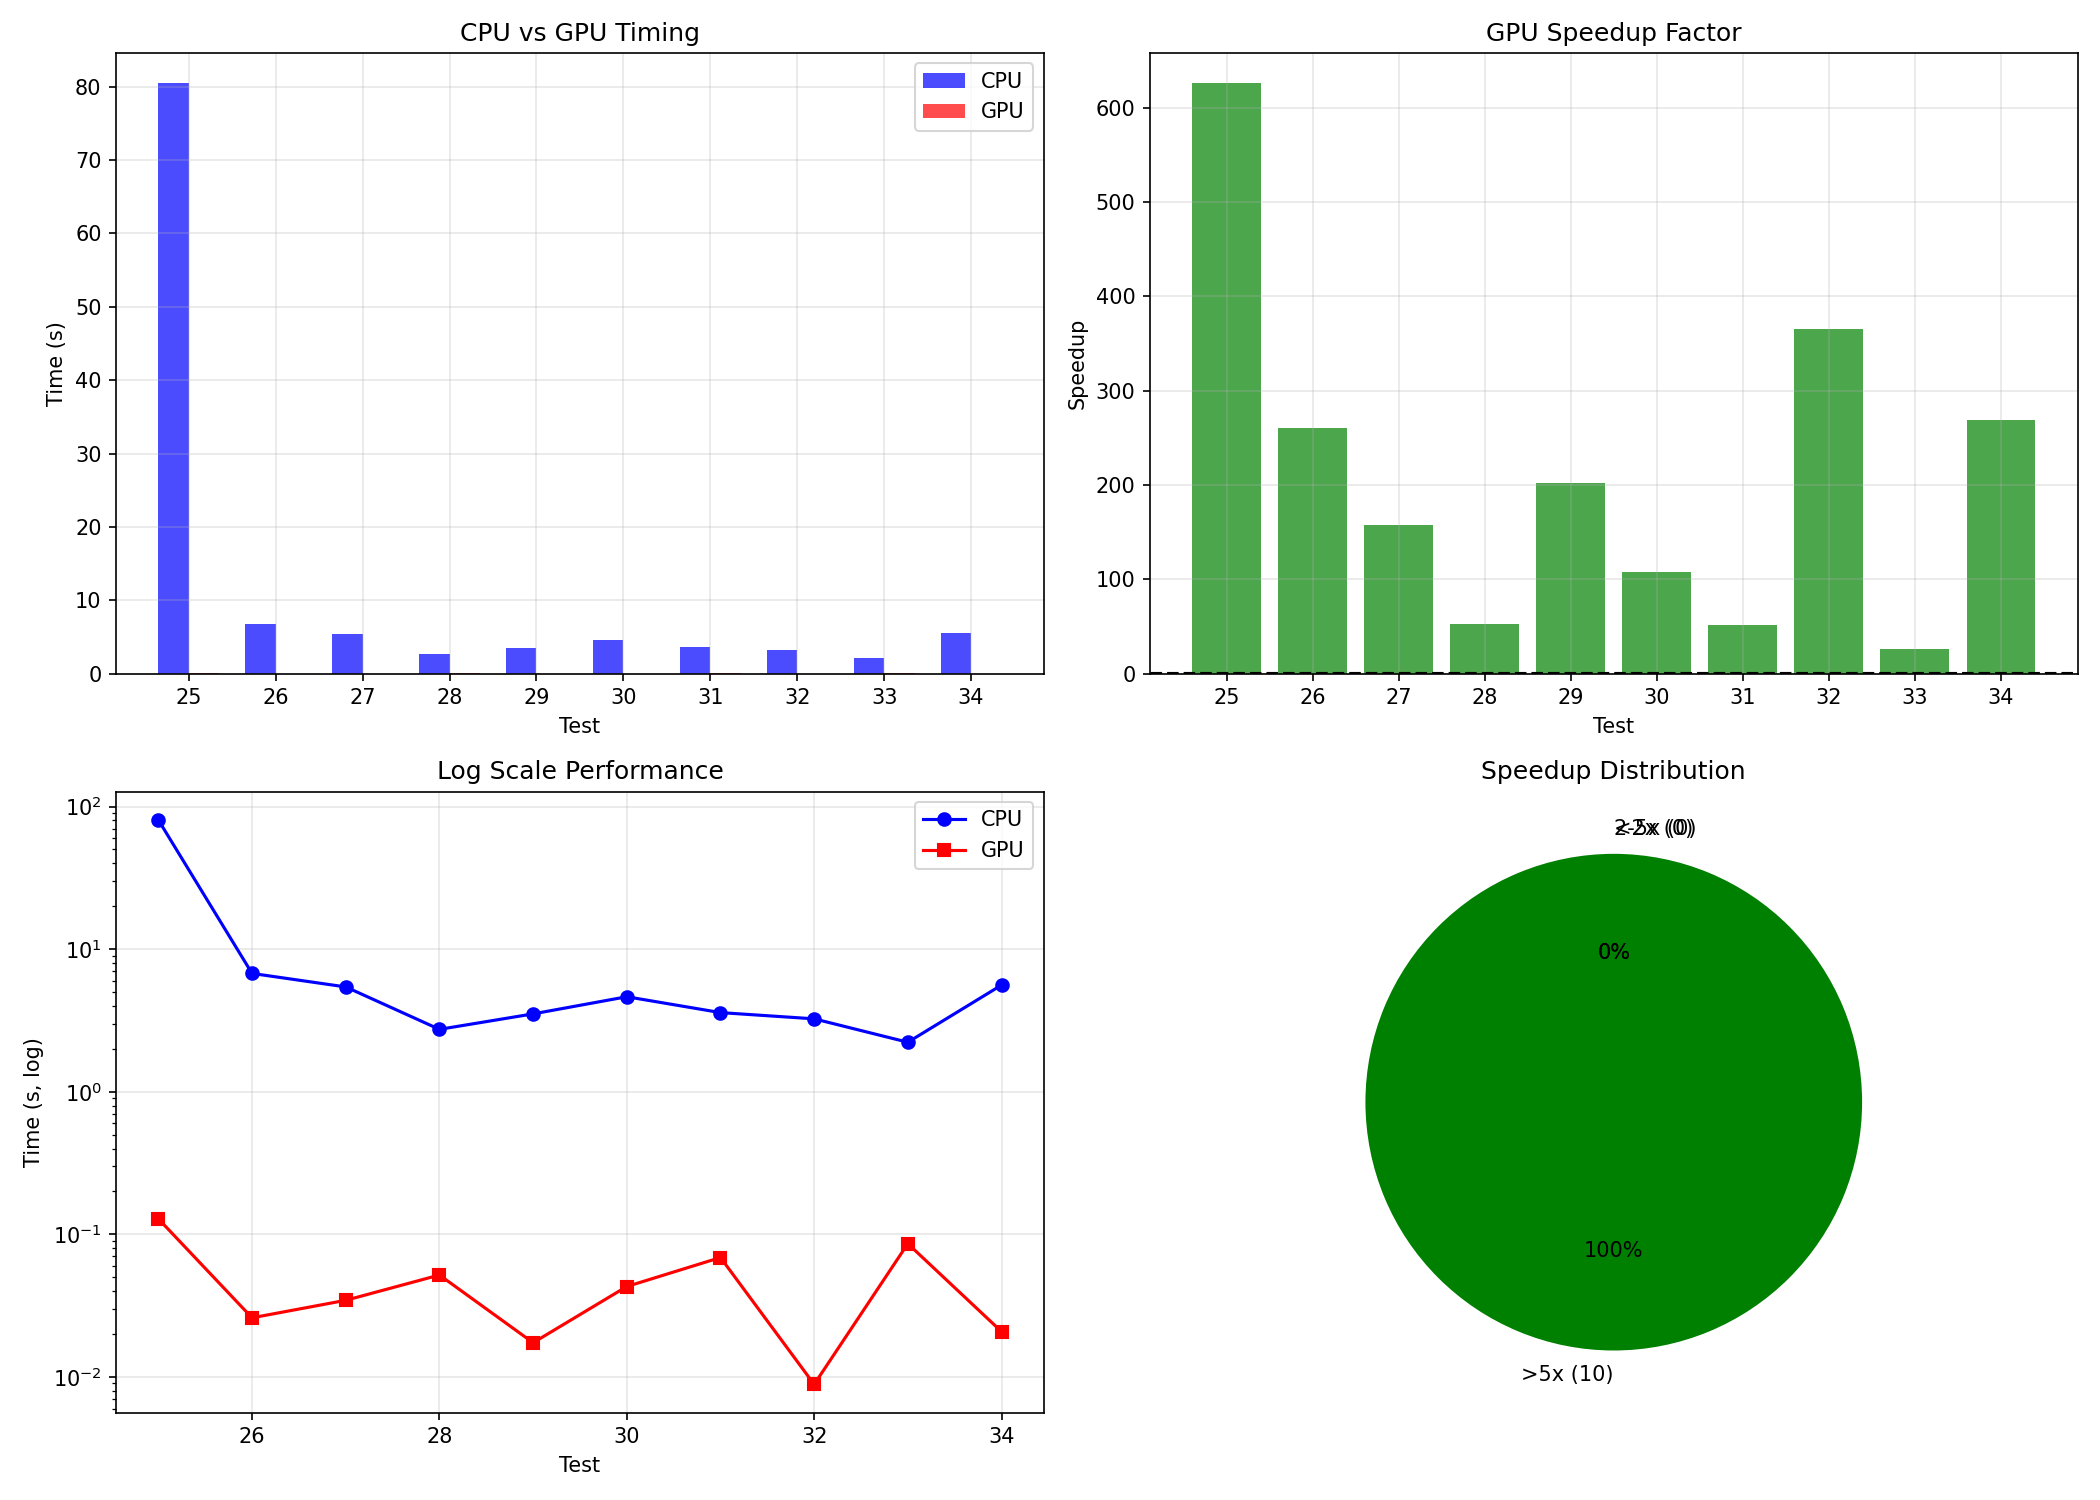
\includegraphics[width=0.9\textwidth]{report_summary.png}
%     \caption{Summary of project achievements including key performance metrics, speedup distribution, and test coverage across different circuit types.}
%     \label{fig:summary}
% \end{figure}

\begin{thebibliography}{9}

\bibitem{ferreira2020}
L. J. S. Ferreira, D. E. Welander, and M. P. da Silva,
``Simulating quantum dynamics with pauli paths,''
arXiv preprint, 2020.

\bibitem{gharibyan2025}
H. Gharibyan, S. Hariprakash, M. Z. Mullath, and V. P. Su,
``A practical guide to using pauli path simulators for utility-scale quantum experiments,''
arXiv preprint arXiv:2507.10771, 2025.

\bibitem{rudolph2024}
M. S. Rudolph,
``PauliPropagation.jl: Julia implementation of pauli propagation,''
\url{https://github.com/MSRudolph/PauliPropagation.jl}, 2024.

\bibitem{qiskit2024}
Qiskit Development Team,
``Qiskit pauli propagation library,''
\url{https://github.com/Qiskit/pauli-prop}, 2024.

% \bibitem{cmu418}
% Carnegie Mellon University,
% ``15-418/618: Parallel computer architecture and programming,''
% Course Materials, Fall 2025.

% \bibitem{nvidia2024}
% NVIDIA Corporation,
% ``CUDA C++ Programming Guide,''
% \url{https://docs.nvidia.com/cuda/cuda-c-programming-guide/}, 2024.

\end{thebibliography}

\section{Work Distribution}

\subsection{Arul Rhik Mazumder (arulm)}

\begin{itemize}
    \item Implemented CPU Pauli propagation algorithm (\texttt{pauli.cpp})
    \item Developed performance benchmarking infrastructure (Python scripts)
    \item Created comprehensive test suite (\texttt{tests.cpp}, 34+ test cases including stress tests)
    \item Performance analysis, visualization, and documentation
\end{itemize}

\subsection{Daniel Ragazzo (dragazzo)}

\begin{itemize}
    \item Designed and implemented CUDA kernel architecture (\texttt{pauli\_gpu.cu})
    \item Implemented device-level gate operations (\texttt{gates.cu\_inl})
    \item Developed parallel prefix sum for truncation (adapted from Assignment 2)
    \item Multi-block coordination and global memory management
    \item GPU debugging, memory optimization, and GHC cluster testing
\end{itemize}

\subsection{Credit Distribution}

\textbf{50\% -- 50\%}

\noindent Both partners contributed significantly to design discussions, debugging sessions, and project direction. The division of implementation work (CPU vs GPU) naturally split responsibilities while requiring close coordination on data structure compatibility and correctness validation.

\end{document}